\documentclass[hyperref={pdfpagemode=UseThumbs, pdfpagelayout=SinglePage, bookmarks=true, },handout,xcolor=dvipsnames]{beamer}

\usetheme{Boadilla}
%\setbeameroption{show notes}
\setbeameroption{show notes on second screen}

\usepackage{url}
\usepackage{hyperref}
\usepackage{amsthm}
\usepackage{amssymb}
\usepackage{mathtools}
\usepackage{float}
\usepackage{tikz}
\usepackage{rotating}
\usepackage{multirow}
\usepackage{graphics}
\usetikzlibrary{arrows,automata,positioning}

\title{\textbf{Automata and Regular Languages}}
\date{\today}

\author{
Oliver
\and
Nam
\and
Michal
\and
Matthew
}

\newcommand{\inputAlphabet}{\mathcal{I}}
\newcommand{\alphabet}{\mathcal{A}}
\newcommand{\aLanguage}{\mathcal{L}}
\newcommand{\automataDef}{(S, S^\prime, \inputAlphabet, T)}
\newcommand{\startStateTable}{\rightarrow}
\newcommand{\acceptStateTable}{\circledcirc}

\begin{document}
\setbeamercovered{transparent}

\begin{frame}
\titlepage

\note{
    (30s): Introduction of members
}
\end{frame}
%\begin{frame}
%\frametitle{Outline}
%\tableofcontents
%\end{frame}
\begin{frame}
\frametitle{``Real World'' Regex}

The following regex finds all phone numbers in all files in the current folder, including PDFs:

\begin{center}
    \textdollar{} rg-all "\^{}(\textbackslash{}+\textbackslash{}d\{1,2\}\textbackslash{}s)?\textbackslash{}(?\textbackslash{}d\{3\}\textbackslash{})?[\textbackslash{}s.-]\textbackslash{}d\{3\}[\textbackslash{}s.-]\textbackslash{}d\{4\}\textdollar{}"
\end{center}

Do not worry if you cannot understand it!

\note{
    (1min): Show an example of a real world regex with syntactic sugar. This could either be a validation regex or bash script regex. Explains what it does briefly. Audience does not need to understand the syntax, this is just for linking theory to practice.

    (style): Dramatic, trying to show off something cool and overwhelm audience with information.
}
\end{frame}
\begin{frame}
\frametitle{Formal regex example}
The following is a formally written regex (without the added syntactic sugar of the real world regex):
\begin{center}
    (A$|$a)a*nn*(y$|$i$|$j$|$h$|$gh)*aa*(h$|$gh)*a*r*s
\end{center}
This one features much less symbols compared to the previous example, although it still looks quite complicated. We will walk you through all the necessary theory to help you understand this.

\note{
    (30s): Gives a cool example of a formally written regex. This should not have any explanation. Regex should be something cool and at the end, what it represents will be revealed.

    (style): Less dramatic, still trying to overwhelm but ease from real world syntax into something that audience might be able to digest.
}
\end{frame}
\begin{frame}
\frametitle{Alphabets, Words, and $\alphabet^*$}
\begin{definition}
    An \textbf{alphabet} is a finite non-empty set containing letters/symbols.
\end{definition}
For example:
\begin{enumerate}
    \item
    The English alphabet
    $$\alphabet = \{A,B,\dots,Z\}$$

    \item
    The binary alphabet
    $$\alphabet = \{0,1\}$$

    \item
    The GBP coin alphabet (in pence)
    $$\alphabet = \{1,2,5,10,20,50,100,200\}$$
\end{enumerate}
\note{
    (2min): Break down the given example into various sections, which are alphabets, words, and A* (explain language and how it is a language is a subset of A*). For each of these concept, show the formal definition on the slides, but spend most of the time doing a run through of an example with the audience. With each of these concept, remember to link back to the example above.

    (style): Change pace depending on whether the audience looks confused or not. In general, go through this slowly while articulating the words clearly. After each concept, pause to let audience have time to think about it. Repeat/ give different example if audience really looks confused.
}
\end{frame}
\begin{frame}
\frametitle{Alphabets, Words, and $\alphabet^*$}
\begin{definition}
    \begin{itemize}
        \item
        A \textbf{word} is a concatenations of letters.
        \item
        An $n$-letter word can be described by the Cartesian product $\alphabet^n$.
        \item
        A special case is the empty word, $\epsilon$.
    \end{itemize}
\end{definition}
\begin{definition}
    The set of all words using an alphabet $\alphabet$ is $\alphabet^* \coloneqq \bigcup\limits_{n \geq 0} \alphabet^n$.
\end{definition}
For example, using the binary alphabet $\alphabet = \{0,1\}$ \\
\begin{itemize}
    \item
    Some possible words are: 001, 100110, 11000110
    \item
    $\alphabet^*$ is the set of all binary strings
\end{itemize}
\note{
Notes from previous slide
}
\end{frame}
\begin{frame}
\frametitle{Languages, Kleene Closure, and Set Operators}
\begin{definition}
    Any subset of $\alphabet^*$ is called a \textbf{language} on $\alphabet$.
\end{definition}
Using the example demostrated on the previous slide where $\alphabet=\{0,1\}$ \\
A possible language on $\alphabet^*$ could be all bit strings that contain an odd number of 1s (odd parity).
\note{
    (2.5min): Keep going to explain language set operators. For each, operator, show how it looks like, link back to formal definition above. With each of these concept, remember to link back to the example above. After laying out the groundwork of operators, show what the precedence of operators is through an example.

    (style): Go through regex operators quickly since these concept are quite straight forward, read the equivalence of each operators in terms of words slowly since this is what we really care about and need.
}
\end{frame}
\begin{frame}
\frametitle{Languages, Kleene Closure, and Set Operators}
\begin{definition}
    $\aLanguage^n$ is defined by $\aLanguage^n=\aLanguage\aLanguage^{n-1}$ $(n \geq 1)$ with $\aLanguage^0=\{\varepsilon\}$
\end{definition}
\begin{definition}
    The \textbf{Kleene closure} of $\aLanguage$ is $\aLanguage^*=\cup_{n \geq 0} \aLanguage^n$.
\end{definition}
\note{
    Notes from previous slide
}
\end{frame}
\begin{frame}
\frametitle{Regex Definitions Using Set Operators}
\begin{definition}
    If r and s are regular expressions over an alphabet $\alphabet
    $ then:
    \begin{enumerate}[i]
      \item $\aLanguage(r^*) = (\aLanguage(r))^*$ (Kleene closure)
      \item $\aLanguage(rs) = \aLanguage(r)\aLanguage(s)$ (concatenation)
      \item $\aLanguage(r|s) = \aLanguage(r) \cup \aLanguage(s) $ (union)
    \end{enumerate}
\end{definition}

\note{
    (30s): Define a regex through the set operators shown.

    (style): Pretending to be bored, read with a dead tone, try to make this funny and basically say that all of this is the culmination of the concept shown above. Allows to go through formal content quickly while keeping attention of the audience.
}
\end{frame}
\begin{frame}
\frametitle{Operator Precedence and Un-parenthesising}

\begin{definition}
    $$\text{(i) } (r^*), \quad \text{(ii) } (rs), \quad \text{(iii) } (r|s),$$
    Order of priority: (i) $\rightarrow$ (iii)
\end{definition}
In any regex, we first do kleene closure, then concatenate and finally do union last.
\\[1em]
For example, take the following regex over the alphabet $\alphabet = \{0,1\}$:

\begin{center}
    $((((0^*)1)|1)(1(1)^*))$
\end{center}

Which, after un-parenthesising the brackets, is the same as:

\begin{center}
    $(0^*1|1)11^*$
\end{center}

\note{
    (1min): Show an example of a regex with more parenthesis as per usual, and go through the act of removing the brackets while explaining why.

    (style): Try to be over the top with the precedence example (as there will be a LOT of brackets).
}
\end{frame}
\begin{frame}
\frametitle{Regex and Specification Regular}
\begin{definition}
    Given an alphabet $\alphabet$, the \textbf{regular expressions} over $\alphabet$, which we denote $\mathcal{R}(\alphabet)$ are strings of symbols from $\alphabet$ augmented by the four special symbols $|$, *, (, and ), (bar, star, parentheses) defined as follows:
    \begin{itemize}
    \item<2-> We have that $\emptyset$, $\varepsilon$, and every element of $\alphabet$ are regular expressions over $\alphabet$
    \item<3-> If $r$ and $s$ are regular expressions over $\alphabet$, then so are the following:
    $$\text{(i) } (r^*), \quad \text{(ii) } (rs), \quad \text{(iii) } (r|s),$$
    \end{itemize}
\end{definition}

\begin{definition}
    Let $\alphabet$ be an alphabet and $\aLanguage$ be a language on $\alphabet$. If there exists a regular expression r on $\alphabet$ that defines $\aLanguage$, then $\aLanguage$ is called \textbf{specification regular}
\end{definition}

\note{
    (1min): Explain specification regular. Say that subset are languages which are specification regular.

    (style): Formal tone, read through the definitions properly.
}
\end{frame}
\begin{frame}
\frametitle{Non-regular Languages: (Informal) Proof}

Finite state machines are just that, \textbf{finite}.
\\[1em]
Languages requiring growing data storage based on input size cannot be encoded. The ``data storage'' in a finite state machine is constant.

\note{
    (30s): Quick informal proof by saying that we cannot have a counting system that counts to infinity because a finite state machines can only store a finite amounts of states.

    (style): Emphasis on the key point of the proof, which is the idea of a FSM only having finite states, while counting goes infinite.
}
\end{frame}
\begin{frame}
\frametitle{Non-regular Languages: Example}

English! You can't create a finite state automata that only accepts correctly written English sentences. We can
hardly approximate that with AI and spellcheckers are still constantly wrong.
\\[1em]
More simply, anything were you might need to ``count'' to arbitrarily large numbers. For example, only accepting
an equation with matching parentheses. e.g. \((()(()))\) but not \((()(())\).

\note{
    (30s): Show an example quickly and explain what we expect it to do and why it breaks.

    (style): Read in a neutral tone, no gimmick here. Normal paced.
}
\end{frame}
\begin{frame}
\frametitle{Diagram of an Automata}
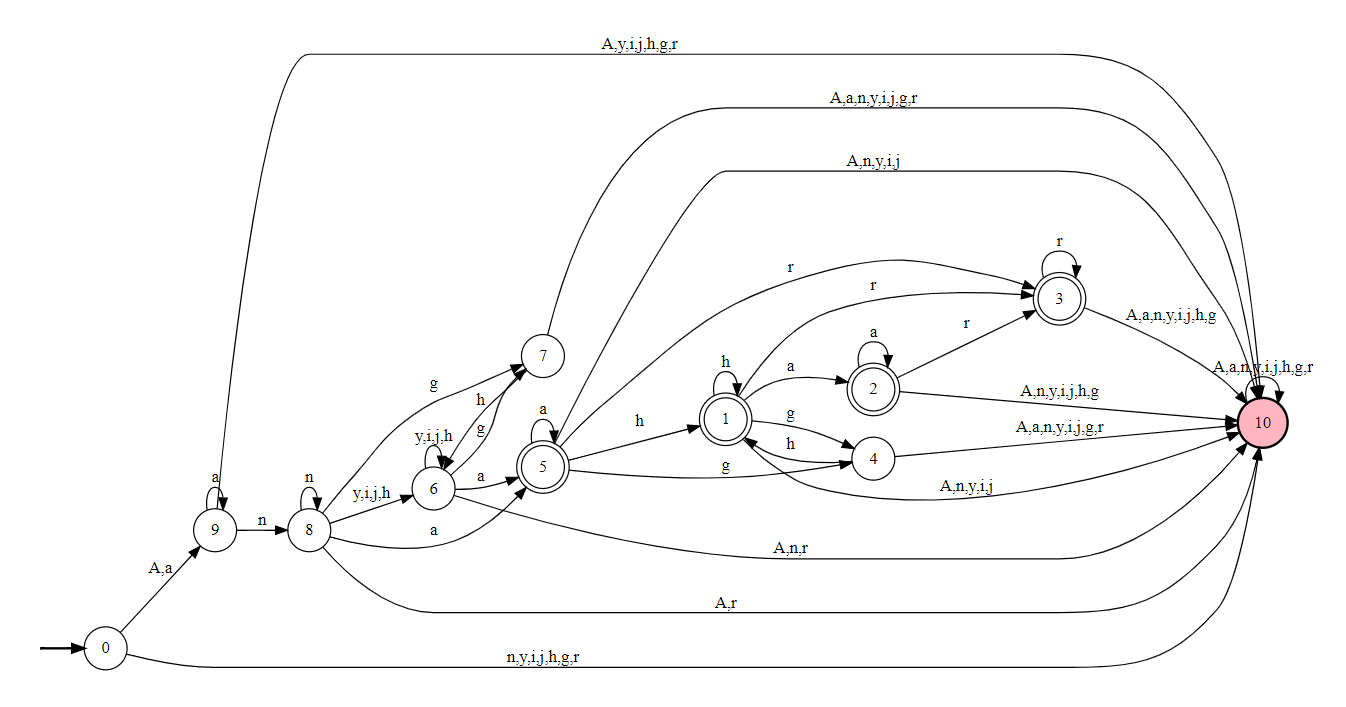
\includegraphics[width=\textwidth]{image.png}

\note{
    (3min): Show an image of a specific automata (this is the equivalent automata of the regex given as the example before). Go through the formal definition of a FSM by pointing out the respective aspect on the diagram (Input alphabet, states, accepting states, transition function). We wont need to go through every single aspect, just show a few and point to where they are on the image.

    (style): Try to impress audience, ``tada'' and such. Tell them how beautiful it is.
}
\end{frame}
\begin{frame}
\frametitle{Transition Table}

\begin{table}
\centering
\resizebox{\textwidth}{!}{
\begin{tabular}{ccc|cccccccc}
	& & \multicolumn{9}{c}{\textbf{Inputs}} \\
\multirow{12}{*}{ \begin{sideways}\textbf{States}\end{sideways} }
	&					&		& A		& a		& n		& y, i, j 	& g		& r 	& h		& $\{A-Z\}\backslash \{A\} \cup \{a-z\}\backslash \{a, n, y, i, j, g, r, h\}$ 	\\ \cline{3-11}
	& $\rightarrow$		& 0	 	& 9 	& 9 	& 10 	& 10 		& 10	& 10	& 10	& 10 	\\
	& $\circledcirc$	& 1		& 10 	& 2 	& 10 	& 10 		& 4		& 3 	& 4		& 10 	\\
	& $\circledcirc$	& 2		& 10 	& 2 	& 10 	& 10 		& 10	& 10 	& 10	& 10 	\\
	& $\circledcirc$	& 3		& 10 	& 10	& 10	& 10		& 10	& 3 	& 10	& 10 	\\
	&					& 4		& 10 	& 10	& 10	& 10		& 10	& 10 	& 1		& 10 	\\
	& $\circledcirc$	& 5		& 10 	& 5		& 10	& 10		& 4		& 3 	& 1		& 10 	\\
	&					& 6		& 10 	& 5		& 10	& 6			& 7		& 10 	& 6		& 10 	\\
	&					& 7		& 10 	& 10	& 10	& 10		& 10	& 10 	& 6		& 10 	\\
	&					& 8		& 10 	& 5		& 8		& 6			& 7		& 10 	& 6		& 10 	\\
	&					& 9		& 10 	& 9		& 8		& 10		& 10	& 10 	& 10	& 10 	\\
	&					& 10	& 10 	& 10	& 10	& 10		& 10	& 10 	& 10	& 10
\end{tabular}
}
\end{table}

\note{
    (30s): Quickly show the transition table which represents the automata above and, again, show which aspect corresponds to the image.

    (style): Boring, go through quickly, say that while this is more useful, the previous one is more beautiful and fun to see.
}
\end{frame}
\begin{frame}
\frametitle{Automata Regular and Regularity}

\begin{definition}
    Let $\alphabet$ be an alphabet and $\aLanguage$ a language on $\alphabet$.
    Then $\aLanguage$ is \textbf{automaton regular} if there exists a finite state automaton $(A,s_0)$
    with $\inputAlphabet = \alphabet$ such that $\aLanguage = \aLanguage(A,s_0)$.
\end{definition}

\begin{definition}
    Let $\alphabet$ be an alphabet and $\aLanguage$ a language on $\alphabet$.
    Then $\aLanguage$ is \textbf{specification regular} if there exists a
    regular expression that describes $\aLanguage$.
\end{definition}

\begin{theorem}
    \[
    \text{\textbf{Automaton regular}} \iff \text{\textbf{Specification regular}}
    \]
\end{theorem}
\note{
    (1min): Define automata regular, and then show that both specification regular and automata regular is equivalent.

    (style): Read in a neutral tone, no gimmick here. Normal paced.
}
\end{frame}

\begin{frame}
\frametitle{Equivalence to Regex}
From what we have just told you above about Automaton regular and specification regular, can you guess what regex  this automaton is equivalent to?

\begin{center}
    (A$|$a)a*nn*(y$|$i$|$j$|$h$|$gh)*aa*(h$|$gh)*a*r*s
\end{center}

Believe it or not, the massive automaton shown above represents the example we gave you right at the start.
\\[1em]
So what does this regex do you? This regex accepts any variation of the name Anna!
\note{
    (30s): Reveal that this is the equivalence of the initial regex!

    (style): Lot of excitement!!!
}
\end{frame}
\end{document}
